\chapter{Porting \textsc{BaseX} to the Android Platform}
\label{sec:migration:porting-basex-to-android}
In the present chapter it is shown how the \textsc{BaseX} database has been migrated to the Android platform.
To achieve this goal the source and target platforms have been analyzed and all necessary requirements have been determined.
The main focus lies on the different software platforms and not on the specific hardware aspects, due to the big variety of systems and devices able to execute both platforms. 
Therefore the two virtual machines and their execution byte formats have been compared and also the specific Android internal mechanisms have been explored.
In Section~\ref{sec:migration:problems-during-the-migration} it is illustrated which parts of the \textsc{BaseX} version have been changed and in which way to receive a working \textsc{BaseX} Android version.
The next section outlines the creation of a client/server architecture using \textsc{BaseX} on the Android operating system.
The last section of the present chapter describes the problems which occurred during the migration process of the database to the Android platform.

\section{Analyzing the Source and Target Platforms} 
\label{sec:migration:analysing-the-source-and-target-platform}
This section outlines the two different platforms and their specific properties.% by analyzing them.
The main part of it concentrates on the software part, because both platforms can be executed on a huge amount of hardware devices.
The term platform is hereby defined as on one side the Java Virtual Machine (JVM) and on the other side the Dalvik Virtual Machine (Dalvik VM, or DVM) in the Android environment.
For a better identification the JVM is marked as the source and the DVM as the target platform.
In later sections the Android operating system is also termed as target platform.
\\
The JVM and the DVM are both virtual machines (VM), but they vary in many different aspects.
To clarify the term virtual machine it has to be said that a VM is a simulated computer, which can be a whole system with all parts a normal computer provides and also needs to execute a program.
Or it is an abstraction layer which provides the functionality to execute a program on every system that runs the virtual machine.
Unlike compiled machine code a program for a virtual machine is platform independent, because it does not matter on which operating system it is executed, as long as the virtual machine is available for the specific operating system.
A disadvantage of this is the loss of speed, which is a result of the execution of the virtual machine and not only the program in general~\cite{craig2006virtual}.
\\
For both virtual machines the programming language Java is used, which is being compiled into code that the VMs understand and are able to execute.
Although both platforms are virtual machines they differ in some crucial ways.
One of the main difference is that the JVM is a stack based and the DVM is a register based virtual machine.
Another distinctness of both machines is that the DVM is optimized to be executed on mobile devices, meaning that it is designed to use less memory and having a low CPU usage than the JVM.
Lesser hardware usage implies also lesser battery usage, which is also a factor which should be considered in the field of mobile development.\\
Another difference, which need to be considered, is the host system, which in case of the DVM only includes Android.
And as opposed to this it could be Windows, Mac OS, or any Linux/Unix derivate as host system running a Java virtual machine. 
This circumstance has to be considered if external resources will be used, like writing or reading a file for example, which is different in every operating system.


\subsection{Comparison of the two Virtual Machines}
\label{sec:migration:comparison-of-the-two-virtual-machines}
As mentioned in the section before both source and target platforms are using Java as its programming language.
Compared to other general purpose programming languages, for example C++, Java is not being compiled into machine code.
To execute Java code a virtual machine is required, that executes the compiled Java code.
However, as in Section~\ref{sec:migration:analysing-the-source-and-target-platform} explained both platforms have different virtual machines.
They differ in many kinds which an application developer not sees but need to consider.
\\
One of the most important differences is that the JVM is a stack and the DVM is a register based virtual machine.
This difference helps the DVM to execute the same code in lesser operations than the JVM.
This means that the DVM need lesser CPU cycles than the JVM, which is an improvement that is necessary due to the lack of CPU and memory resources in mobile devices and the aspect of battery usage.
This can be demonstrated by comparing the instructions done by adding two integers in both virtual machines.
The stack based virtual machine has to execute four machine instructions, while the register based VM is able to do the same operation in one single instruction.
The reason for this is that the stack based VM needs to pop the two values first before it can add and store them back on the stack.
The instructions included in the example operation for the stack based machine are \textit{'pop 1', 'pop 2', 'add 1 2', 'push result'}.\\
Figure~\ref{fig:stack-based-addition} illustrates the instruction steps which need to be performed to execute an addition with a stack based virtual machine.
\begin{figure}[h]
\begin{center}
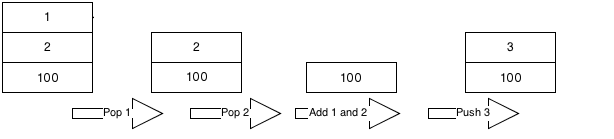
\includegraphics[scale=0.65]{images/stack-based-addition.png} 
\caption{The addition of two integers on a stack based virtual machine.}
\label{fig:stack-based-addition}
\end{center}
\end{figure}
\newpage
Compared to this, the register based virtual machine just needs one single machine instruction to complete the same addition of two numbers.
The required instruction for this task is \textit{'ADD R1, R2, R3'}, which can be translated into: add the contents of register 1 and register 2 and store the result in register 3.
Figure~\ref{fig:register-based-addition} illustrates this by showing the add operation of the numbers '1' and '2'.
\begin{figure}[h]
\begin{center}
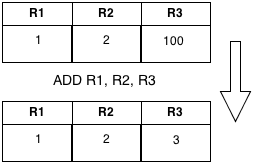
\includegraphics[scale=0.65]{images/register-based-addition.png} 
\caption{The addition of two integers on a register based virtual machine.}
\label{fig:register-based-addition}
\end{center}
\end{figure}

This minimal example shows how the register based virtual machine uses lesser machine instructions compared to the stack based.
The disadvantage in this approach of a register based machine is that it has to store the addresses, meaning the corresponding registers, of the operands.
Which is not necessary at a stack based machine because the stack pointer always directs to the actual operand using the Last In First Out (LIFO) principle.
This leads to the result, that stack based code is smaller than the equivalent register based code.
Although the Dalvik VM is a register based virtual machine, the executed byte code is not bigger than the equivalent JVM code~\cite{shi2008virtual}.\\
This is the result of the different formats of the executable virtual machine code, which is optimized in the case of the Dalvik virtual machine and is illustrated later in Chapter~\ref{sec:comparison-of-the-two-bytecode-formats}.
\\
The code that represents the instructions which are executed on Dalvik VM or the JVM is called bytecode.
To execute bytecode instructions virtual machines having an interpreter which interprets all instructions and performs them.
The difference to normal interpreted languages is, that the JVM or DVM interpreters do not need to check the syntax of a program.
This has already been done by the Java compiler which compiles the Java source code into so called class files.
Even if it is faster than other interpreted languages, it is still slower than code that is compiled into a certain machine language and executed directly on the hardware.
This so called machine code is faster because there is no layer between the executions and the hardware, which could slow down the execution~\cite{aycock2003brief}.\\
There is a technique which can significantly improve a virtual machine in performance aspects by adding a Just In Time (JIT) compiler to it.
In general it can be said, that a JIT compiler, used by a virtual machine, compiles heavy used code segments or very expensive calculations into a much faster machine code.
There is a great number of different types of JIT compilers and how they work, the two used by the JVM or the DVM are:
\begin{itemize}
\item method-based
\item trace-based
\end{itemize}
The trace-based method works by looking at the most executed code fragments, especially loops, and compiles them into native machine code.\\
The method-based JIT mechanism, in contrast to the trace-based, compiles whole methods, which are often used and expensive in execution time, into native machine code.
Since the release of the Android version 2.2, release name Froyo, the Dalvik VM has received a JIT compiler additionally to the interpreter mechanism.
According to Cheng~\cite{cheng2010jit} the implemented Dalvik JIT compiler can speed up the execution of intensive operations up to five times.
The Dalvik VM uses the above mentioned mechanism of a trace-based JIT compiler mixed with its usual interpreter.
The given advantage of the trace-based method is that not whole methods are being compiled into machine code.
Instead only the parts which are often executed are being compiled.
This reduces the size of the code which needs to be compiled by the JIT and also omits the not so often executed methods parts like exception handling.
It is needles to compile such parts in machine code to speed them up, because most of the execution time of the program they are not being called.
This should also reduce the compile time of the JIT, because of the selective compilation into machine code.\\
To realize this the Dalvik virtual machine has received an additional thread, which is responsible for the JIT compilation.
Beneath this new thread there is the main thread, that includes the interpreter.
This interpreter interprets the bytecode and records the traces and their occurrences.
If the amount of the occurrence is higher than a predefined number, the trace is being stored into the trace queue.
The new added thread, the JIT thread, compiles the traces from the queue and writes the machine code into the code cache.
The main thread now is doing a lookup if the bytecode that needs to be executed is available in the code cache, at the moment.
If this condition is met, it uses the machine code from the code cache instead of interpreting the actual bytecode~\cite{oh2012evaluation}.
Picture~\ref{fig:dvm-threads} illustrates the principle of the two threads inside the DVM.\\
\begin{figure}[h]
\begin{center}
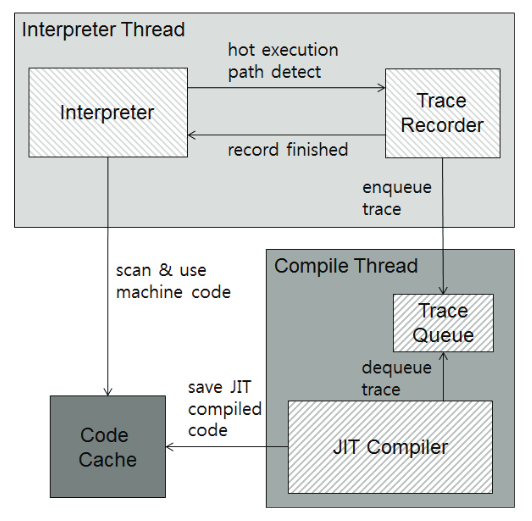
\includegraphics[scale=0.5]{images/dvm-threads.png} 
\caption{The principle of the two DVM threads. Source:\cite{oh2012evaluation}}
\label{fig:dvm-threads}
\end{center}
\end{figure}
\newpage
Depending on the different implementation of a JVM, it differs in the way which type of JIT compiler mechanism is used.
For this thesis the Oracle JVM \textit{HotSpot} is used, which has a method-based JIT compiler as default.
But it is also possible to use another JIT mechanism in the \textit{HotSpot} JVM triggered by parameters during the VM start.
The method-based JIT works as mentioned above, it compiles the most called methods into machine code~\cite{kotzmann2008design}.
Those methods are called hot spots, which are also responsible for the name of the virtual machine~\cite{paleczny2001java}.
\\
Both virtual machines are providing a garbage collector, which is responsible for the memory management of the executed bytecode.
Same as the principle of an own instance of the Dalvik virtual machine per process, which will be explained in Section~\ref{sec:android-internals}, every process also has its on instance of a garbage collector on Android.
It is a mark-and-sweep garbage collector that only collects the objects that are not referenced any more inside the application heap.
The shared heap, which is part of the Zygote process, and which is also described in Section~\ref{sec:android-internals}, has its own garbage collector~\cite{maia2010evaluating}.
\\
Although both virtual machines are using Java as programming language, Dalvik lacks of some libraries that are available for the JVM and vice versa.
In Section~\ref{sec:migration:migration-of-basex-to-android} the libraries used by the \textsc{BaseX} database are analyzed and investigated which of them are supported by the DVM.\\
An overall statement about both virtual machines could not be made, because the fact that they differ in many aspects.
Especially considering that the DVM has been created for the mobile context and can only be ran on Android devices\footnote{Some community projects exist which are aiming to port the Dalvik VM to other platforms like Linux x86. For example the Android x86 project: \url{http://www.android-x86.org/}}.



\subsection{Comparison of the two Bytecode Formats}
\label{sec:comparison-of-the-two-bytecode-formats}
Both virtual machines also differ in their usage of formats for the executable files.
On one side there is the Java Archive File (JAR) for the JVM and on the other side the Dalvik Executable (\textit{dex}).
The \textit{dex} is being packed into an Android Application package file (\textit{apk}) which can be executed by the Android operating system.
A JAR file is an archive which includes the compressed class files. 
These class files are being build out of the Java source code by using the \textit{javac} compiler~\cite{pugh1999compressing}.
An \textit{apk} file is also an archive file, but it does not only include the executable program, it also includes the meta information and resource files.
Although an Android application is an \textit{apk} file only the format of the \textit{dex} file is outlined here, due to the fact that the DVM executes those files.
A \textit{dex} file is created by using a tool which compiles Java class files into \textit{dex} files.
This tool is called \textit{dx} and it is part of the Android software development kit.
Picture~\ref{fig:create-apk} illustrates the flow of creating an \textit{apk} file, which differs from the creation of a JAR file by creating the \textit{dex} files out of the class files before packing them into an archive.\\
\begin{figure}[h]
\begin{center}
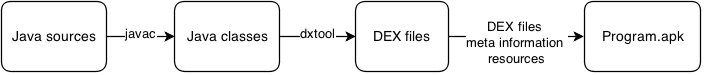
\includegraphics[scale=0.55]{images/create-apk.png} 
\caption{The creation flow of an \textit{apk} file.}
\label{fig:create-apk}
\end{center}
\end{figure}

Having a closer look at the \textit{dex} files and comparing them to the JAR files shows that they differ in various ways.
The first thing that comes in mind is that a JAR file contains a class file for every Java class.
Compared to this a \textit{dex} file combines all specific information into one field.
This is realized by just having one constant pool, in which all constant values of all classes are stored.
These constants consist of:
\begin{description}
  \item[string\_ids] Sorted list of all string identifiers
  \item[type\_ids] Sorted list of all class identifiers, arrays or primitive data types
  \item[proto\_ids] Sorted list of all prototypes
  \item[field\_ids] Sorted list of all identifiers for the used fields
  \item[methods\_ids] Sorted list of all methods used by the \textit{dex} file
\end{description}
Considering an interface which is used very often in a project can outline what advantage is given with the use of one shared constant pool.
Looking at Image~\ref{fig:jar-dex} demonstrates that every class which uses this interface has to have a reference within its own constant pool only and not the whole constant pool as itself.
\begin{figure}[h]
\begin{center}
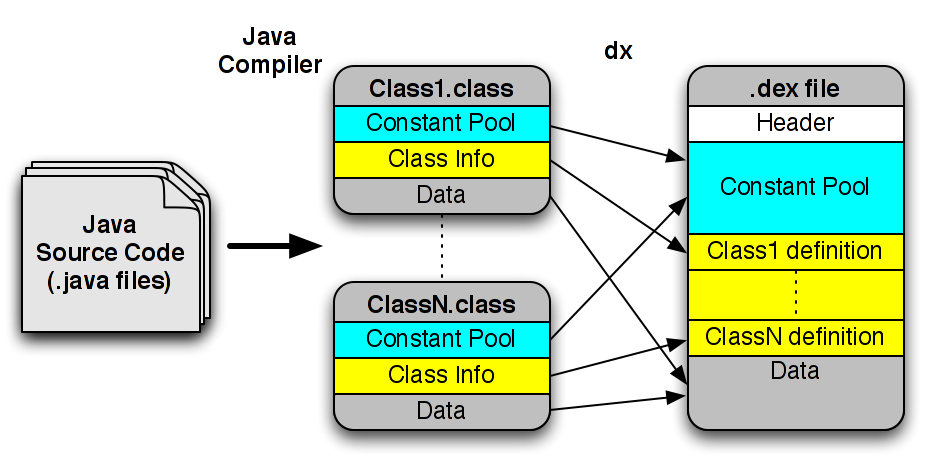
\includegraphics[scale=0.41]{images/jar-dex.png} 
\caption{The difference between a jar and a \textit{dex} file. Source:\cite{enck2011study}}
\label{fig:jar-dex}
\end{center}
\end{figure}

In general it can be said that \textit{dex} files are smaller than their equivalent JAR files, because of using this shared constant pool~\cite{bornstein2008dalvik}.
An advantage of the creation chain of a \textit{dex} file is that it is theoretically possible to create a \textit{dex} file out of every jar archive.
The problem hereby is that Android does not support all Java libraries that the JVM supports, but this can be passed over by using the above mentioned dx-tool. 
As already said before, a \textit{dex} file is executed by the Dalvik virtual machine, but it is not the Android application.
An Android application is the \textit{apk} file that also includes user interface related information and other resource files, like images or sound files.

\subsection{\textsc{BaseX} Internals}
\label{sec:migration:basex-internals}
Although \textsc{BaseX} can be executed on every system that offers an implementation of the Java virtual machine, it has its specialties depending on the operating system that is used.
This is the case if there is something about storing files on the file system.
\textsc{BaseX} stores its databases and configuration files in a folder in the home directory of the user.
This folder is created by the database if it does not exist yet.\\
Hence, \textsc{BaseX} has to figure out on which operating system it is running.
After \textsc{BaseX} knows of the underlying operating system it stores several operating system specific information inside a static class, which is called \textit{Prop}. 
This class needs to be adjusted during the migration process.
One value inside this class is used to indicate if the path name is case sensitive, which is only relevant for a Linux or Unix operating system and not for Windows or Mac.
To store its databases inside the folder in the directory of the home directory of the current user \textsc{BaseX} needs the absolute path to this specific folder.
Therefore the static Java system method \textit{System.getProperty(``user.home'')}, which returns the absolute path to the home directory of the user on a normal JVM, is used.\\
Another difference between Windows and other Unix based operating systems is that Windows uses a backslash ``\textit{$\backslash$}'' as path separator instead of a usual slash.
This information is also stored inside the above mentioned \textit{Prop} class by using the static Java system method \textit{System.getProperty(``line.separator'')}.

\subsection{Android Internals}
\label{sec:android-internals}
As shown in the Sections~\ref{sec:migration:comparison-of-the-two-virtual-machines} and \ref{sec:comparison-of-the-two-bytecode-formats} the two virtual machines and their corresponding bytecode formats differ.
However, Android has some other specialties about its internal processing procedure.
The Android operating system is a Linux based operating system aimed to run on mobile devices.
Therefore it has been created as a Linux fork of the 2.6.*\footnote{Since Android version 4.* a Linux kernel 3.* is used} kernel and it has been especially designed for the mobile context.
This includes a special focus on the resource consumption, because most mobile devices do not provide the same resources as a normal desktop PC or a notebook does.
As shown in Section~\ref{sec:migration:comparison-of-the-two-virtual-machines} an Android application is executed in the Dalvik virtual machine.
At this point it has to be said that every application runs its own instance of the Dalvik VM, by forking the main Dalvik instance into an own Linux process.
Here the Android policy sets in, where every application is independent from any other application and is executed in its own process, which is called sandbox.
This principle also applies for all locations of files the application needs and uses.
An application is similar in its rights and processing to a user in the Linux operating system.
Every application is its own user and uses its own home directory.
This directory can only be accessed by the owning application and is located in the /data/data system directory.
This system directory can include its own SQLite3 database, cache directory, shared preferences\footnote{Android framework that provides a mechanism to store primitive data types.} and every type of private data.
The aspect of security is the reason for this type of solution as well as the stability of the application, considering the own Dalvik instance.
This is called the \textit{principle of least privilege} which specifies that privileges as less as possible are given to the application.
Therefore application developers have to specify which privileges their application need, for example Internet access or the possibility to write on the external SD-card.
It is possible that applications can communicate with predefined Inter-process Communications (IPC) but it is not possible to manipulate other applications.
This can be omitted by granting root privileges to an application, but usually this is not possible on normal distributed devices.
Hence, confidential data should also be encrypted, because theoretically it is possible to access the data inside the private directory.
It also need to be said that every operation which reads or writes to one of the above mentioned directories or files is an input output (I/O) operation.
This is always expensive in time consumption and should be done as little as possible.
Image~\ref{fig:zygote-and-app} illustrates the principle that every application works in its own sandbox.\\
\begin{figure}[h]
\begin{center}
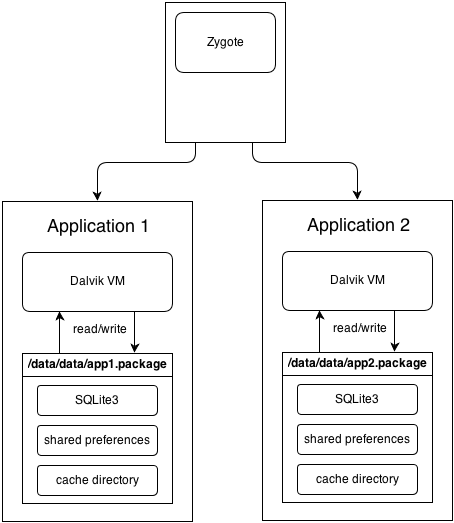
\includegraphics[scale=0.75]{images/zygote-and-app.png} 
\caption{Illustration of the Android application architecture}
\label{fig:zygote-and-app}
\end{center}
\end{figure}

The main Dalvik instance, which is the root parent for all forked virtual machines, is called Zygote and it is started by the boot up process of Android.
Zygote is designed to load and initialize the core library classes so that every forked instance does not have to do this on its own.
This is compared to starting a new virtual machine a speed improvement and saves memory, because not every VM instance has to have its own core libraries loaded.
This can be done because the core libraries are all read only and are shared by all Dalvik instances~\cite{ehringer2010dalvik}.
Another difference to the usual Linux operating system is that Android uses the \textit{Bionic libc} which is a special from Google developed library for Android, which has its own \textit{pthread} implementation.
This library is especially designed for the mobile context and the Android environment which improves the speed of forking the Dalvik virtual machine too.~\cite{brady2008android}

\section{Migration of \textsc{BaseX} to Android}
\label{sec:migration:migration-of-basex-to-android}
After analyzing both platforms the \textsc{BaseX} database code also needs to be examined.
Like it has been mentioned in Section~\ref{sec:migration:comparison-of-the-two-virtual-machines} the Dalvik virtual machine does not support all class libraries that are supported by the JVM.
\textsc{BaseX} is written in the Java programming language and aims to be executed on virtual machines that are implemented by using the JVM specifications.
Therefore it is not possible to transform the \textsc{BaseX} jar file into a \textit{dex} file, using the dx-tool, and execute it on an Android device.
On the other hand the DVM offers class libraries that the JVM does not support or is really aware of.
These libraries do not intent to replace not supported Java class libraries.
Their solely purpose is to provide special Android related methods, like logging or tracing of method calls as well as accessing hardware components of a mobile device, sensors or the mobile network for example. 

\subsection{Analyzing the Libraries used by \textsc{BaseX}}
\label{sec:migration:analyzing-the-libraries-used-by-basex}
\textsc{BaseX} is a big project which consists of up to 60 packages and more than 1300 classes, interfaces and abstract classes.
For this reason the examining of the used libraries and the dependencies a special tool was used: the so called Class Dependency Analyzer (CDA)\footnote{http://www.dependency-analyzer.org/}. 
It offers all needed possibilities for the mentioned task.\\
Parsing the whole \textsc{BaseX} project lists the used Java class libraries and external libraries.
This list consists of 54 packages that are part of the Java class library or an external library used by \textsc{BaseX}.
It has to be supposed that none of them are known to the Dalvik virtual machine.\\
Most of them represent subpackages of given packages and it can be expected that if a main package is not supported by Android its subpackages are neither.
This assumption reduces the external packages to a total number of 16, which is compared to the before mentioned 54 packages an easier to analyze amount.
Looking at the Android documentation the main packages that are not supported are just the two graphical user interface (GUI) related packages:
\begin{itemize}
	\item \textsf{java.awt}\footnote{Except the subpackage java.awt.font that provides two classes: NumericShaper and TextAttribute.} and
	\item \textsf{javax.swing}
\end{itemize}
All other packages are fully or at least partially supported by the Java language of the Dalvik VM.
The reason why the packages \textsf{awt} and \textsf{swing} are not supported is that Android uses its own GUI libraries and framework.
The Android provided GUI elements can either be written as Java code or can be defined in specific XML layout files, which get used to created the corresponding Java files during the compile process.
The framework offers everything that is needed to build an application with a graphical user interface.\\
Supporting the other main packages does not mean that all subpackages, classes or even included methods that are used from other libraries are also known by the DVM.
Therefore more investigation needs to be done in order to get a better overview of the supported packages.
To get a clearer statement about the given situation, the subpackages are also being checked if they are supported by the DVM or not.
The result of this investigation shows that \textsf{javax.xml} is supported, but not the following subpackages:
\begin{itemize}
	\item \textsf{javax.xml.crypto.dom}
	\item \textsf{javax.xml.crypto.dsig.dom}
	\item \textsf{javax.xml.crypto.dsig.keyinfo}
	\item \textsf{javax.xml.crypto.dsig.spec}
\end{itemize}
Even if all packages and classes of \textsf{javax.xml.crypto} are part of the Java standard edition they are not available for Android development.
All classes inside this packages are only used by one single \textsc{BaseX} package, which is called \textsf{org.basex.query.\-util.crypto}.
This package is used to implement the XQuery cryptographic module that provides functionalities to en- and decrypt, sign and validate signed XML data.
The only class that makes use of this package is the \textsf{FNCrypto} class.
This class is used to provide the cryptographic module functionalities in XQuery.
These are XQuery functions which consist of:
\begin{itemize}
	\item \textsf{hmac(string,string,string[,string])}
	\item \textsf{encrypt(string,string,string,string)}
	\item \textsf{decrypt(string,string,string,string)}
	\item \textsf{generate-signature(node,string,string,string,string,string[,item][,item])}
	\item \textsf{validate-signature(node)}
\end{itemize}
To provide these five XQuery functions for Android, the \textsf{javax.xml.crypto} package needs to be migrated to Android, too.
Another possibility to support these XQuery functions would be the use of other cryptographic classes which are provided by Android.\\
All other subpackages that are not directly mentioned are supported by the Android platform.
For clarification not all methods that are provided by every used library are checked whether they are available for Android.
This process would be to much effort, considering the high amount of available classes.
Nevertheless this will be figured out in Section~\ref{sec:migration:creating-a-basex-android-library} and Section~\ref{sec:migration:problems-during-the-migration} outlines the methods which are not supported by different versions of Android.

\subsection{The Android Project Structure}
\label{sec:migration:the-android-project-structure}
For developing Android applications an Android project needs to be set up initially.
An Android project is a structure of special folders and predefined files, like code, resource and build files.
There are three types of Android projects, which are differing in their functionalities and intentions.\\
The first is the type of project that needs to be created if an executable application is the goal of the development process.
As a result of this an installable \textit{apk} file will be created during the build process.\\
The second type of Android project specifies the so called Test project.
This type of project aims to test executable Android projects by providing an Android testing framework including unit test, using the Java unit test framework \textit{JUnit}.
Both projects have the identical structure of folders and files.\\
The third project type represents the library project which goal it is to be a library that can be used by every other Android project.
The difference to a normal Android project lies in the fact that this project is not being build into an \textit{apk} file.
Instead it is being used by other Android projects which pull it in their respective \textit{apk} file and build it with their code.
Depending on the specific Android API level an Android library differs from a usual Java library, by the fact that the Android library is not compressed into a jar archive.
This feature has been added in Android versions higher than API level 14(Android 4.0 codename Icecream Sandwich).
For older versions, before this API level, the library files were pulled into the project and compiled into the corresponding \textit{dex} file.\\
If a new Android application is developed it is not necessary to set up the right project structure by hand.
Therefore Android provides a Software Development Kit (SDK).
This SDK provides tools and utilities to create each of the three types of a Android project.
It also includes build, debug, trace and test tools.
With this SDK, which is also called Android Developer Tools (ADT), it is possible to create Android applications written in Java.
As it was mentioned in Section~\ref{sec:comparison-of-the-two-bytecode-formats}, the code that is translated into bytecode for the Dalvik virtual machine is written in the Java programming language.
Though, it is also possible to write code in C++ and compile it into native code, like it is done by the, referred in Section~\ref{sec:migration:comparison-of-the-two-virtual-machines}, JIT mechanism.
Therefore Google provides an Android Native Development Kit (NDK), that offers tools and a specific compiler to translate such native C++ code.
If a project has been successfully created there are seven given folders, shown in Table~\ref{tab:android-project-folders}.
\begin {table}[htpb] 
  \centering
\begin {tabular} {|l|l|}
	\hline
	Folder&Content\\
	\hline
	src/&The Java source code files\\
	\hline
	bin/&The compiled output file\\
	\hline
	jni/&C++ native code created by using the NDK\\
	\hline
	gen/&Automatically generated Java files\\
	\hline
	assets/&Every kind of file, which needs to be packed into the \textit{apk} file as it is\\
	\hline
	res/&All XML resource files\\
	\hline
	libs/&The Private libraries\\
	\hline
\end {tabular}
\caption {Android project folders generated by the SDK.}
\label {tab:android-project-folders}
\end {table}

The files that will be generated while creating an Android project consists of four build files that each holds information used by the build system to create the \textit{dex} files and the \textit{apk} archive.
Another file that is being created is the so called \textit{AndroidManifest.xml}.
This XML file is important for the application and the Android operating system.
It is used to specify the API level, the application name and other specific information related to the application.
In this file it is also possible to grant privileges to the application that are needed for specific functionalities.
For example accessing the Internet or writing on an external storage card.
Libraries used within the project are also defined in this file.
But if a referenced library is in need of specific privileges and defines them inside its own mainfest file, they are not automatically granted by Android.
Therefore it is necessary to manually grant these privileges in the Android project and not in the library project, because declarations made inside a library manifest are being ignored.


\subsection{Creating a \textsc{BaseX} Android Library}
\label{sec:migration:creating-a-basex-android-library}
For the migration of \textsc{BaseX} to the Android operating system a library project has been created.
The reason to make \textsc{BaseX} as Android library, as explained in Section~\ref{sec:migration:the-android-project-structure}, is that Android libraries can be used by many other projects.
After creating the library project all \textsc{BaseX} files have been copied to this project.
After this operation the GUI packages have been removed, those packages are \textsf{basex.gui} and all subpackages of it.
As a result the depending classes of the GUI have also been removed.
Those are also not necessary because the \textsc{BaseX} Android library does not need to provide a graphical user interface.
Afterwards the not supported \textsf{javax.xml.crypto} packages and the dependent class \textsf{FNCrypto} have been removed.
Therefore it not possible to use the cryptological XQuery function in the Android version of \textsc{BaseX}.\\
The result of removing all not supported packages, classes and libraries leads to the fact that it is possible to compile \textsc{BaseX} to an Android \textit{dex} file, at this point.
Although it is not possible at this moment to execute \textsc{BaseX}, because of some constraints, mentioned in Section~\ref{sec:android-internals}, and not facing the fact that an Android library is not executable.\\
In a usual Linux environment \textsc{BaseX} stores all its database files inside a directory in the normal user directory.
This means executing \textsc{BaseX} on Android without adjusting the directory to store the databases, would not work.
\textsc{BaseX} receives the name and location of the home directory of the user by calling the Java function \textit{System.getProperty(``user.home'')}, which works well with the JVM.
Using this function on Android returns an empty string and results in \textsc{BaseX} trying to save the database in the root directory, what is impossible, because of the Android right system explained in Section~\ref{sec:android-internals}.
To avoid this behavior the above mentioned function needs to be replaced.
The path where the data has to be stored must be a directory that only the application can access.
Every application receives one directory with the given constraint from Android.
This is where it will be installed as well as where the application will store its data.
Additionally to this it is possible for an application to read or write on external storage, but this is not protected by the operating system which means that every application is able access and modify those files.\\
The problem by using the private application directory is that \textsc{BaseX} should be a library project and it should be usable by every other Android project.
So it is impossible to say how the directory is named and to locate where the database files have to be stored before even knowing how the application, which uses the \textsc{BaseX} library, is called.
The explanation for this is that an Android application receives its directory by the name of its main package and not by the name of the library main package, so that more than one application can use this library.
This is an issue that has to be dealt with, which is illustrated and discussed later in Section~\ref{sec:migration:problems-during-the-migration}.
Hence, it is necessary to tell the library this location and use it instead of its own package name.
To implement this behavior a class has been created which is an entry point for the library.
And it is the first instance when the \textsc{BaseX} Android library is used.
This class creates an object of the library and needs the package name of the application as an argument for the method that returns an instance of its object.
To create the object the Singleton pattern has been used~\cite{gamma2010entwurfsmuster}.
The reason for this is that only one instance of the database can be created and used inside one application.\\
This class is called \textsf{BaseXDatabase} and creates a \textsc{BaseX} Context object by calling a constructor that has been added to the Context class.
The newly created Context constructor checks if the given directory is available and if it is possible to read and write to this directory.
Is it the first time the constructor of the class is used, it creates a directory which is called \textsf{BaseXData}.
All databases created and used by this Android application are stored inside this directory.
The directory is only accessible from this application\footnote{Assuming the application is executed on a non rooted device.}.
At this moment it is possible to use \textsc{BaseX} as an Android library and it would create the needed \textsc{BaseX} directory.\\
To provide the \textsc{BaseX} operations the above mentioned class has been extended by additional methods which can be used for this purpose.
All are implemented by using the above mentioned Context object, which means every operation is executed on this object.\\
After the migration process it is possible to use \textsc{BaseX} as it can be done on every usual PC which provides an implementation of the JVM.
Except the cryptographic XQuery function, the \textsc{BaseX} Android library offers all functionalities like the normal \textsc{BaseX} desktop version offers.
The Android principle that every application works in its own sandbox is also being kept.
With this type of solution every application has its own \textsc{BaseX} database in its own directory.
A possible advantage of this result is that the database does not need to consider queries that are coming from another application and synchronizations of the queries.\\
However, in the next section an alternative solution to this is provided by implementing the client/server mechanism of \textsc{BaseX} in Android.
The advantages and disadvantages of the library implementation are outlined and investigated in Chapter~\ref{cha:analysis}.
For the validation and performance measurement a test application of the \textsc{BaseX} Android library has been written and its execution performance analyzed, illustrated in Section~\ref{sec:analysing-the-execution-performance}.

\subsection{Providing a \textsc{BaseX} Android Client/Server Solution}
\label{sec:migration:providing-a-server-client-solution}
At this moment every application which uses the \textsc{BaseX} Android library, has its own database which is able to create, read, update and delete the data.
One disadvantage of that type of solution is that other applications are not able to use the data inside a database of another application.
The reason for this, as mentioned in Section~\ref{sec:android-internals}, is the sandbox principle of Android applications where applications can only access their own resources and not those from other applications.
Speaking of a disadvantage could be misleading in this context, because this circumstance also prevents unauthorized applications to read or modify the data of another application.
However, Android provides a mechanism which offers the possibility to provide data from one application to another.
This technique is called Content Provider and is used for system wide databases like the database that contains the contacts of the owner of an Android device.
Thinking of different applications that are using the same data shows that this could lead to redundant databases, which would increase the required storage size.
In addition to this, every time the data changes on one point it has to be synchronized with every other database which stores the same data, too.
For example, if every application has its own database storing the contacts and a new contact is added, all those databases need to updated.\\
Additionally to the stand alone version of \textsc{BaseX} it is possible to use it as a client/server solution.
An instance of a \textsc{BaseX} client connects to a server and sends its requests and queries to it, which executes them and sends them back to the client.
The advantage of this solution is that the client does not have to do the execution of the database related operations.
Also the files which are containing the data, are stored and managed on the server and not on the client.
Both shown advantages are reducing resource consumptions at the client instance.
It also saves storage size as well as execution resources like the CPU or RAM occupation.
But there is also a disadvantage, namely the client can only operate if there is a server available, and therefore it needs a connection to the server to send requests and receive responses.\\
As mentioned in Section~\ref{sec:overview:introduction-into-basex} \textsc{BaseX} also provides a client/server solution, which also has been migrated to the Android platform.
Hereby the focus does not lie on the execution of the server on an external device, like a server on the Internet for example.
Although this is also possible and would result in a big saving of resources on the mobile device, but this would be similar to a web service which is not the focus of this thesis.
The server client architecture of the Android \textsc{BaseX} version is to have one central database on one place and one instance of a server that handles all the upcoming database operations.
In contrast to the, as outlined in the section before, Android library there is only one place on the device where the respective database files are being stored.
If an application wants to use \textsc{BaseX} as a database it uses the client that sends the operations to the server, which is executed on the same device, and then receives the results.
To achieve this Android provides Inter Process Communication (IPC) mechanisms which are offering the possibility to communicate between different applications.\\
However, the client/server version of \textsc{BaseX} uses the network and the TCP protocol to do the communication between server and clients.
This technique has also been used for the Android solution of the client and server implementation.
Additionally the server has been created as an Android service.
An Android service is a process which is executed in the background and is thus the last instance which is killed by Android process management.
The reason to implement the server as an Android service is the process management of the operating system and the execution of the service in the background of the device.
The constraint of limited RAM forces the Android process management to kill the not needed application and free their used spaces inside the RAM~\cite{developers2011android}.
This can not be controlled, and the server has to be available all the time, so that an application can do its operation in exchange with it.
The Android operating system tries to keep the service as long as possible alive, depending on different criteria and even it is being killed, for example by the user, it tries immediately to restart it.
A service does not provide a graphical user interface and to communicate with it also IPCs are used.
As for this an application has been written, to start and stop the server service.
This application also has its own sandbox where the server stores its data.
The application as well as the background service are executed in this sandbox.
The data is stored in this sandbox, so no other application can access the data inside it, therefore the server is used.
To achieve this goal \textsc{BaseX} uses, as well as the desktop version, the network for the communication with the clients.
Specifically the client application does not need to implement IPCs, they send their requests via the network to the server and also receive the responses through the network.
A graphical illustration of this principle is shown in Figure~\ref{fig:server-client-android}.

\begin{figure}[h]
\begin{center}
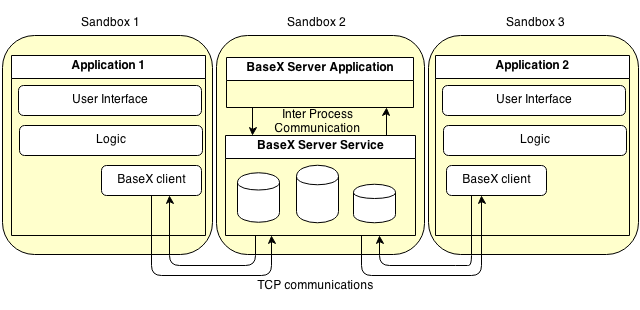
\includegraphics[scale=0.6]{images/basex-server-client.png} 
\caption{The principle of the \textsc{BaseX} server client communication in Android.}
\label{fig:server-client-android}
\end{center}
\end{figure}

Every request and operation, which uses the \textsc{BaseX} client/server model, is executed on the device and thus there is no saving in execution resources, only in storage capability if different applications are using the same data.
The implementation of the client server mechanism for Android has been done to illustrate that it is possible to have a server and client of \textsc{BaseX} running on one single device.
The implication of this section is that it is also possible to have an external server which provides the data and handles the execution of any operation, which saves the above mentioned resources at the client.
The only way to provide application data to another application is given when using the so called content providers supplied by Android itself.
The \textsc{BaseX} client/server implementation could also be seen as an alternative for the present Android content providers.\\
\\
Additionally the \textsc{BaseX} Android client as well as the library implementation are both implementing the same interface, so it is easy to replace one version with the other.
This makes it easy to replace the library with the client solution if the resources have to be stored somewhere else, for example on an external server.



\section{Problems During the Migration}
\label{sec:migration:problems-during-the-migration}
During the migration of \textsc{BaseX} to the Android operating system several problems and issues occurred.
The first problem which was discovered, was, as mentioned in Section~\ref{sec:migration:analyzing-the-libraries-used-by-basex}, the lack of some included libraries, that are not supported by Android.
To solve this issue they have been removed and their functionality has been deprecated.
This has been done, because those specific functionalities are not required for a first runnable Android version of \textsc{BaseX}. 
This also applies for all graphical user interface components, which also have been removed, because they are not necessary for an Android library.\\
Another problem was the location of the \textsc{BaseX} database directory on the Android device.
This need to be, as already described in Section~\ref{sec:android-internals}, the \textit{/data/data/app\-lication-package-name} directory.
The problem hereby is that one of the goals of the migration process is that the database is a library and not a standalone application.
In the Android operating system the name of the private directory of an application depends on the name of its main package.
This is only available if there is an Android application. 
A library does not offer this type of information, so it is not possible for a library to get the name or location of its private directory.
The only way to get the package name of the application, except of hard coding it into the source code, is to get the application context and extract the name from there.
This bears another problem, though only applications have a context, libraries do not, which also need to be considered. 
A possible way, could be to pass the context to the library, but then the library holds the context which it does not usually need and it will maybe not be freed from the garbage collector, due to the mark-and-sweep garbage collector strategy, as described in Section~\ref{sec:migration:comparison-of-the-two-virtual-machines}.
Also the library would only need the application context to receive the application name and by using this information the name and location of the private directory.
As mentioned above, holding an Android context massively slows down an Android application, so this is not the way how the problem should be solved.
The alternative is to pass a string holding the application name to the constructor of the library, because it only needs the name or the location of the \textit{data/data} directory to access it.
Therefore the context has been used before creating a library instance to receive the needed directory name, so that it can be passed right to the library through the constructor.
The string, containing the directory name, then is used by the library to generate the needed directories.
This can be done by the library, because it directly belongs to the application that uses it.
As a result of this the library is executed in the same sandbox like the application and it has the corresponding rights.
%This is also the way how it is done in the \textsc{BaseX} library, as it was described in Section~\ref{sec:migration:creating-a-basex-android-library}.\\
An issue with this solution is that the user directory which is used inside \textsc{BaseX} is a static string value initialized at the start of \textsc{BaseX}.
All static values used by \textsc{BaseX} are initialized at start-up from within the static class \textsf{Prop}.
And right after the start \textsc{BaseX} uses this value from this class in several places in the code.
Which means that it need to be changed before it is being used anywhere in the code.
For this reason a trick has been used to initialize the value before the constructor calls another constructor.
In the \textsc{BaseX} \textit{Context}\footnote{This is the \textit{BaseX} Context class, and not the Context class, mentioned above, which is provided by Android.} class the constructor which calls the actual constructor has been changed to initialize this value as a parameter.
This results in the cycle of constructor calls, that the constructor which is called initializes the static values before calling the upcoming constructor in the chain.
The corresponding Java code can be seen in Listing~\ref{lst:context-constructor}.
The reason the file separator is not determined by using the available system method \textsf{System.getProperty(``line.separator'')} lies in the fact that the used separator is the same as in Linux.
Namely it is the normal slash ``/'' and not a backslash as it is implemented inside the Windows operating systems.

\lstset{language=Java,
   basicstyle=\footnotesize,
   keywordstyle=\color{blue!80!black!100},
   identifierstyle=,
   commentstyle=\color{green!50!black!100},
   stringstyle=\ttfamily,
   breaklines=true,
   numbers=left,
   tabsize=2,
   numberstyle=\footnotesize,
   frame=single,
   backgroundcolor=\color{blue!3},
}
\begin{lstlisting}	[captionpos=b, captionpos=b, caption={The constructor of the BaseX context class.}, label=lst:context-constructor] 		        	   
public Context(String data_dir) {
  this(true, (Prop.HOME = data_dir + ``/''), (Prop.USERHOME = data_dir + ``/''));
        	
  File dir = new File(Prop.HOME + ``BaseXData'');
  if(!dir.exists()) {
    if(!dir.mkdir()) {
     android.util.Log.i(``BASEX'', ``CREATING BASEX DIRECTORIES'');
    }  
  }
}
\end{lstlisting} 


Another issue which occurred during the migration process, was that \textsc{BaseX} intensively uses the Java string function \textsf{isEmpty()}, which is not available at an Android API-level lower than 9.
The same applies for the \textsf{copyOf()} method in the \textsf{java.util.Arrays} Java package.
This issue was solved by not supporting API-levels lower than 9 with the created \textsc{BaseX} library.
According to the official Android homepage only 1.7\% of the devices that are currently in circulation have an API-level lower than 9.\footnote{\url{http://developer.android.com/about/dashboards/index.html}}
As a consequence developers can only create applications that are executable on Android devices using an API-level higher than 9, while using the \textsc{BaseX} library.
To assure that no application, that is build on Android version lower than 9, uses the \textsc{BaseX} library the Manifest file of the library has been adjusted.
This applies to one of the cases where the Manifest file of a library is used to determine the minimum Android version.
Other constraints specified inside this Manifest file, like write permissions for example, are being ignored, as it was mentioned in Section~\ref{sec:migration:the-android-project-structure}.

